
\documentclass[11pt]{article}
\usepackage[margin=1in]{geometry}
\usepackage{caption} %For captioning objects
\usepackage{subcaption} %sub-captioning pictures
\usepackage{graphicx} %to include graphics
\usepackage{hyperref} %for clickable references
\usepackage{listings} %to write code listings
\lstset{language=R, breaklines=true}  
\usepackage[mathcal]{euscript} %for curly S
\usepackage{mathtools}
\usepackage{float} %so figures can be placed "here"

%Defining commands for math symbols
\usepackage{amsmath} %to enable split equations
\usepackage{statmath} %for plim. Be careful, it has already \E and \V.
\usepackage{amssymb} %to enable mathbb
\newcommand{\R}{\mathtt{R}} %Software R
\renewcommand{\E}{\mathbb{E}} %expectation
\usepackage{bbm}
\newcommand{\1}{\mathbbm{1}}
\renewcommand{\V}{\mathbb{V}} %variance
\newcommand{\N}{\mathcal{N}} %normal distribution
\newcommand{\U}{\mathcal{U}} %normal distribution
\renewcommand{\P}{\mathbb{P}} %proba, renewcom since \P already exists
%Regression variables in vector form
\newcommand{\y}{\boldsymbol{y}} 
\newcommand{\x}{\boldsymbol{x}} 
\newcommand{\z}{\boldsymbol{z}} 
\newcommand{\yhat}{\boldsymbol{\hat{y}}} 
\renewcommand{\u}{\boldsymbol{u}} 
\newcommand{\uhat}{\boldsymbol{\hat{u}}}  
\newcommand{\Px}{\boldsymbol{P}}  
\newcommand{\Mx}{\boldsymbol{M}}  
\newcommand{\A}{\boldsymbol{A}}  
\newcommand{\X}{\boldsymbol{X}}  
\newcommand{\Z}{\boldsymbol{Z}}  
\newcommand{\e}{\boldsymbol{e}}  
\renewcommand{\r}{\tilde{r}}  
%\renewcommand{\r}{\boldsymbol{r}} 
\renewcommand{\i}{\boldsymbol{\imath}} 
\newcommand{\alphab}{\boldsymbol{\alpha}}  
\newcommand{\betab}{\boldsymbol{\beta}}  
%opening

\newcounter{daggerfootnote}
\newcommand*{\daggerfootnote}[1]{%
	\setcounter{daggerfootnote}{\value{footnote}}%
	\renewcommand*{\thefootnote}{\fnsymbol{footnote}}%
	\footnote[2]{#1}%
	\setcounter{footnote}{\value{daggerfootnote}}%
	\renewcommand*{\thefootnote}{\arabic{footnote}}%
}


\title{Problem Set 3 - ECON 880\\
	\small Spring 2022 - University of Kansas}
\author{Gunawan, Minh Cao}


\begin{document}

\maketitle	

\section*{Problem 1}
In this exercise, we are interested in solving $Ax=b$, where
\[A = \begin{pmatrix}
	54 &14& -11& 2 \\ 14 &50& -4& 29 \\ -11 &-4 &55& 22 \\ 2& 29& 22& 95
\end{pmatrix}, \quad b = \begin{pmatrix}
	1\\1\\1\\1
\end{pmatrix} \]
using Gauss-Jacobi and Gauss-Seidel method. Both methods yield the same result
\[x = \begin{pmatrix}
	0.0189\\
	0.0168\\
	0.0234\\
	-0.0004
\end{pmatrix}.\]
Gauss-Jacobi method required 0.0207 seconds with 45 iterations until convergence. The residual is given by
\[
10^{-11} \times \begin{pmatrix}
	0.0361\\
	-0.1211\\
	-0.0922\\
	0.2351
\end{pmatrix}
\]
Gauss-Seidel method required 0.0193 seconds with 23 iterations until convergence. The residual is given by
\[10^{-12}\times \begin{pmatrix}
	0.1013\\
	-0.1849\\
	-0.1201\\
	-0.0002
\end{pmatrix}\]
   
\section*{Problem 2}
In this exercise, we are interested in solving $Bq=r$ using extrapolation, where

\[B = \begin{pmatrix}
 1&0.5&0.3\\0.6&1&0.1\\0.2&0.4&1
\end{pmatrix}, \quad r = \begin{pmatrix}
	5\\7\\4
\end{pmatrix}. \]
Following Ken Judd's definition\daggerfootnote{Kenneth L. Judd, 1998. "Numerical Methods in Economics," MIT Press Books, The MIT Press, p.78-79}, we first define $G=I-B$, and run the following iteration
\[q^{k+1}=\omega G q^k +\omega r + (1-\omega)q^k,\] 
where we pick $\omega=1.05$, tolerance level $10^{-13}$, and initial value $q_0=(0,0,0)'$. The extrapolation converged after $k=97$ iterations, with the residual 
\[Bq-r =  10^{-12} \times
\begin{pmatrix}
0.1670\\
-0.2371\\
0.1279
\end{pmatrix}.\] 
The solution to the linear equation system is
\[
q=\begin{pmatrix}
	1.6716\\
	5.8651\\
	1.3196
\end{pmatrix}
\]
\section*{Problem 3}
We want to solve the following functions 
\begin{enumerate}
	\item $\sin(2\pi x)-2x=0$
	\item $\sin(2\pi x)-x=0$
	\item $\sin(2\pi x)-0.5x=0$
\end{enumerate}
using 1) Bisection, 2) Newton method, 3) Secant method, and 4) fixed-point iteration. We want to evaluate for what value of initial guess $x_0\in[-2,2]$ these methods converge. We proceed by first plotting all the three functions on Figure \ref{fig:3}. From these graphs, we see that within the interval $[-2,2]$, function 1 and 2 have both two roots, while function 3 has seven roots.

\begin{figure}[htbp]
	\centering
	\begin{subfigure}[b]{0.48\textwidth}
		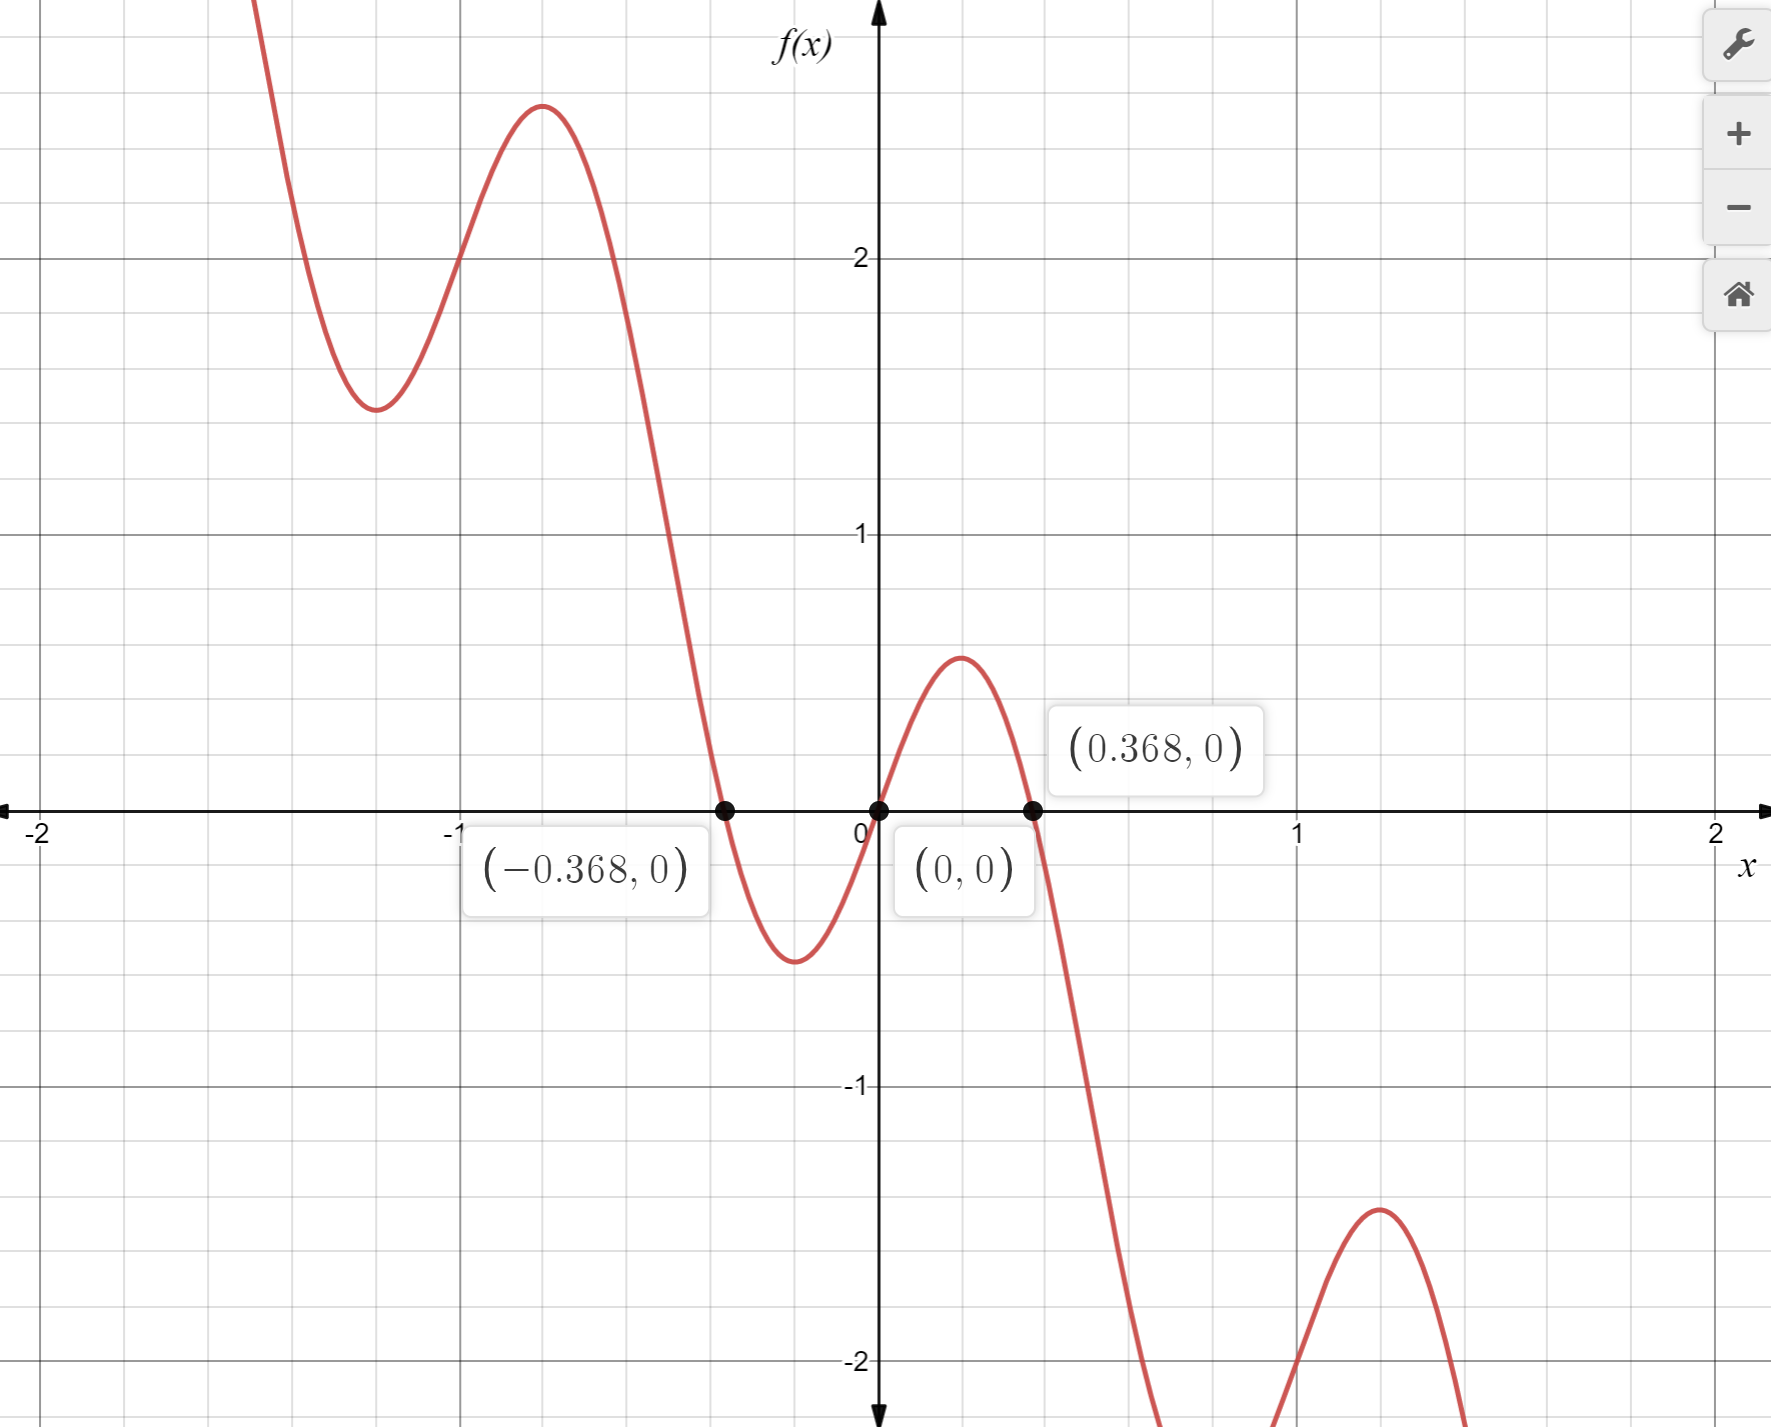
\includegraphics[width=\textwidth]{f1.png}
		\caption{$f(x)=\sin(2\pi x)-2x$}
		\label{3a}
	\end{subfigure}
	~
	\begin{subfigure}[b]{0.48\textwidth}
		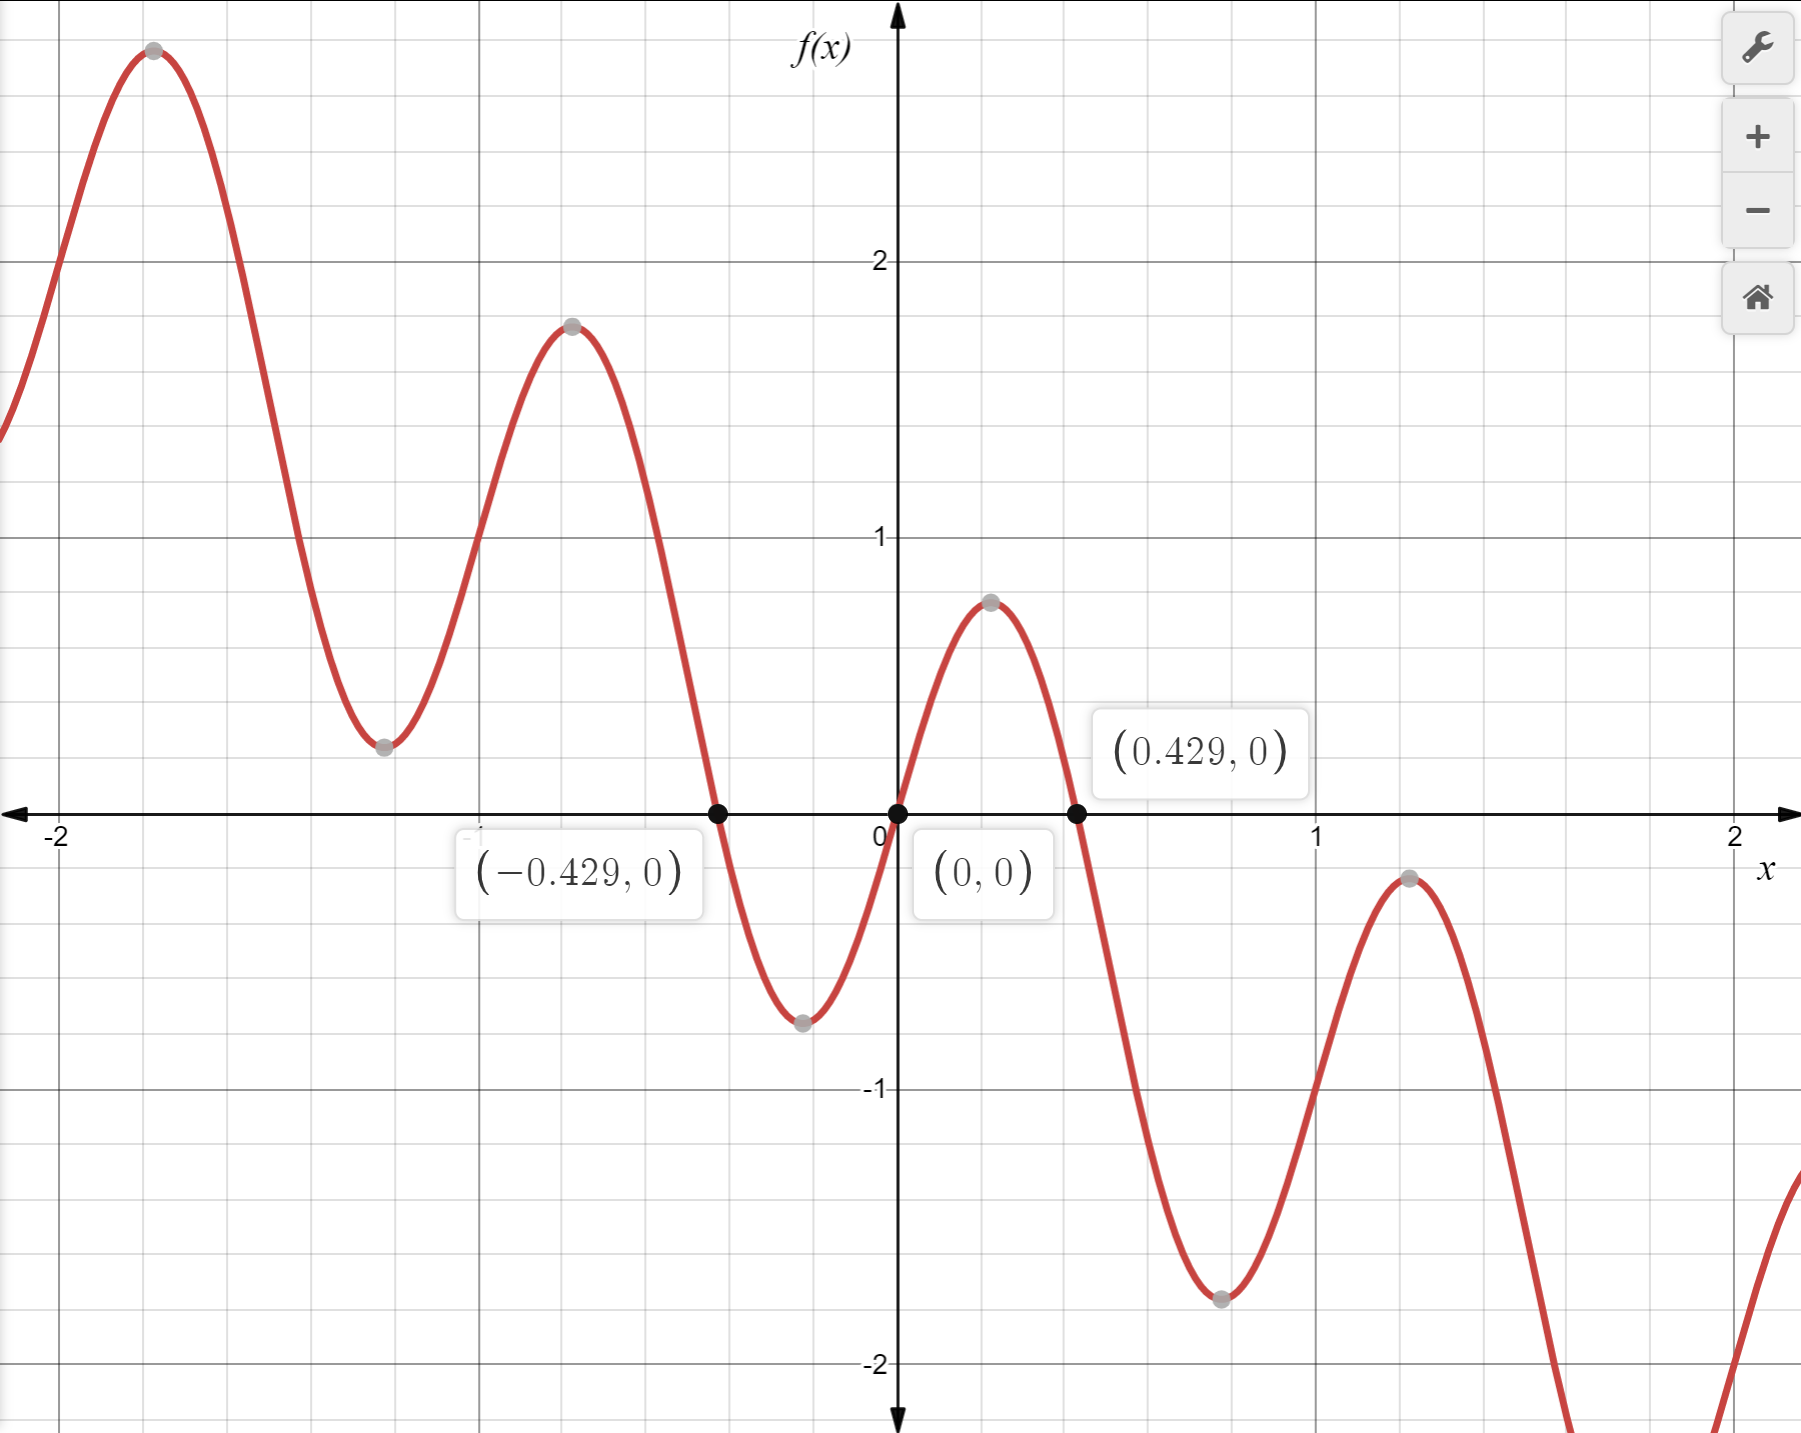
\includegraphics[width=\textwidth]{f2.png}
		\caption{$f(x)=\sin(2\pi x)-x$}
		\label{3c}
	\end{subfigure}
	\newline
	\begin{subfigure}[b]{0.48\textwidth}
		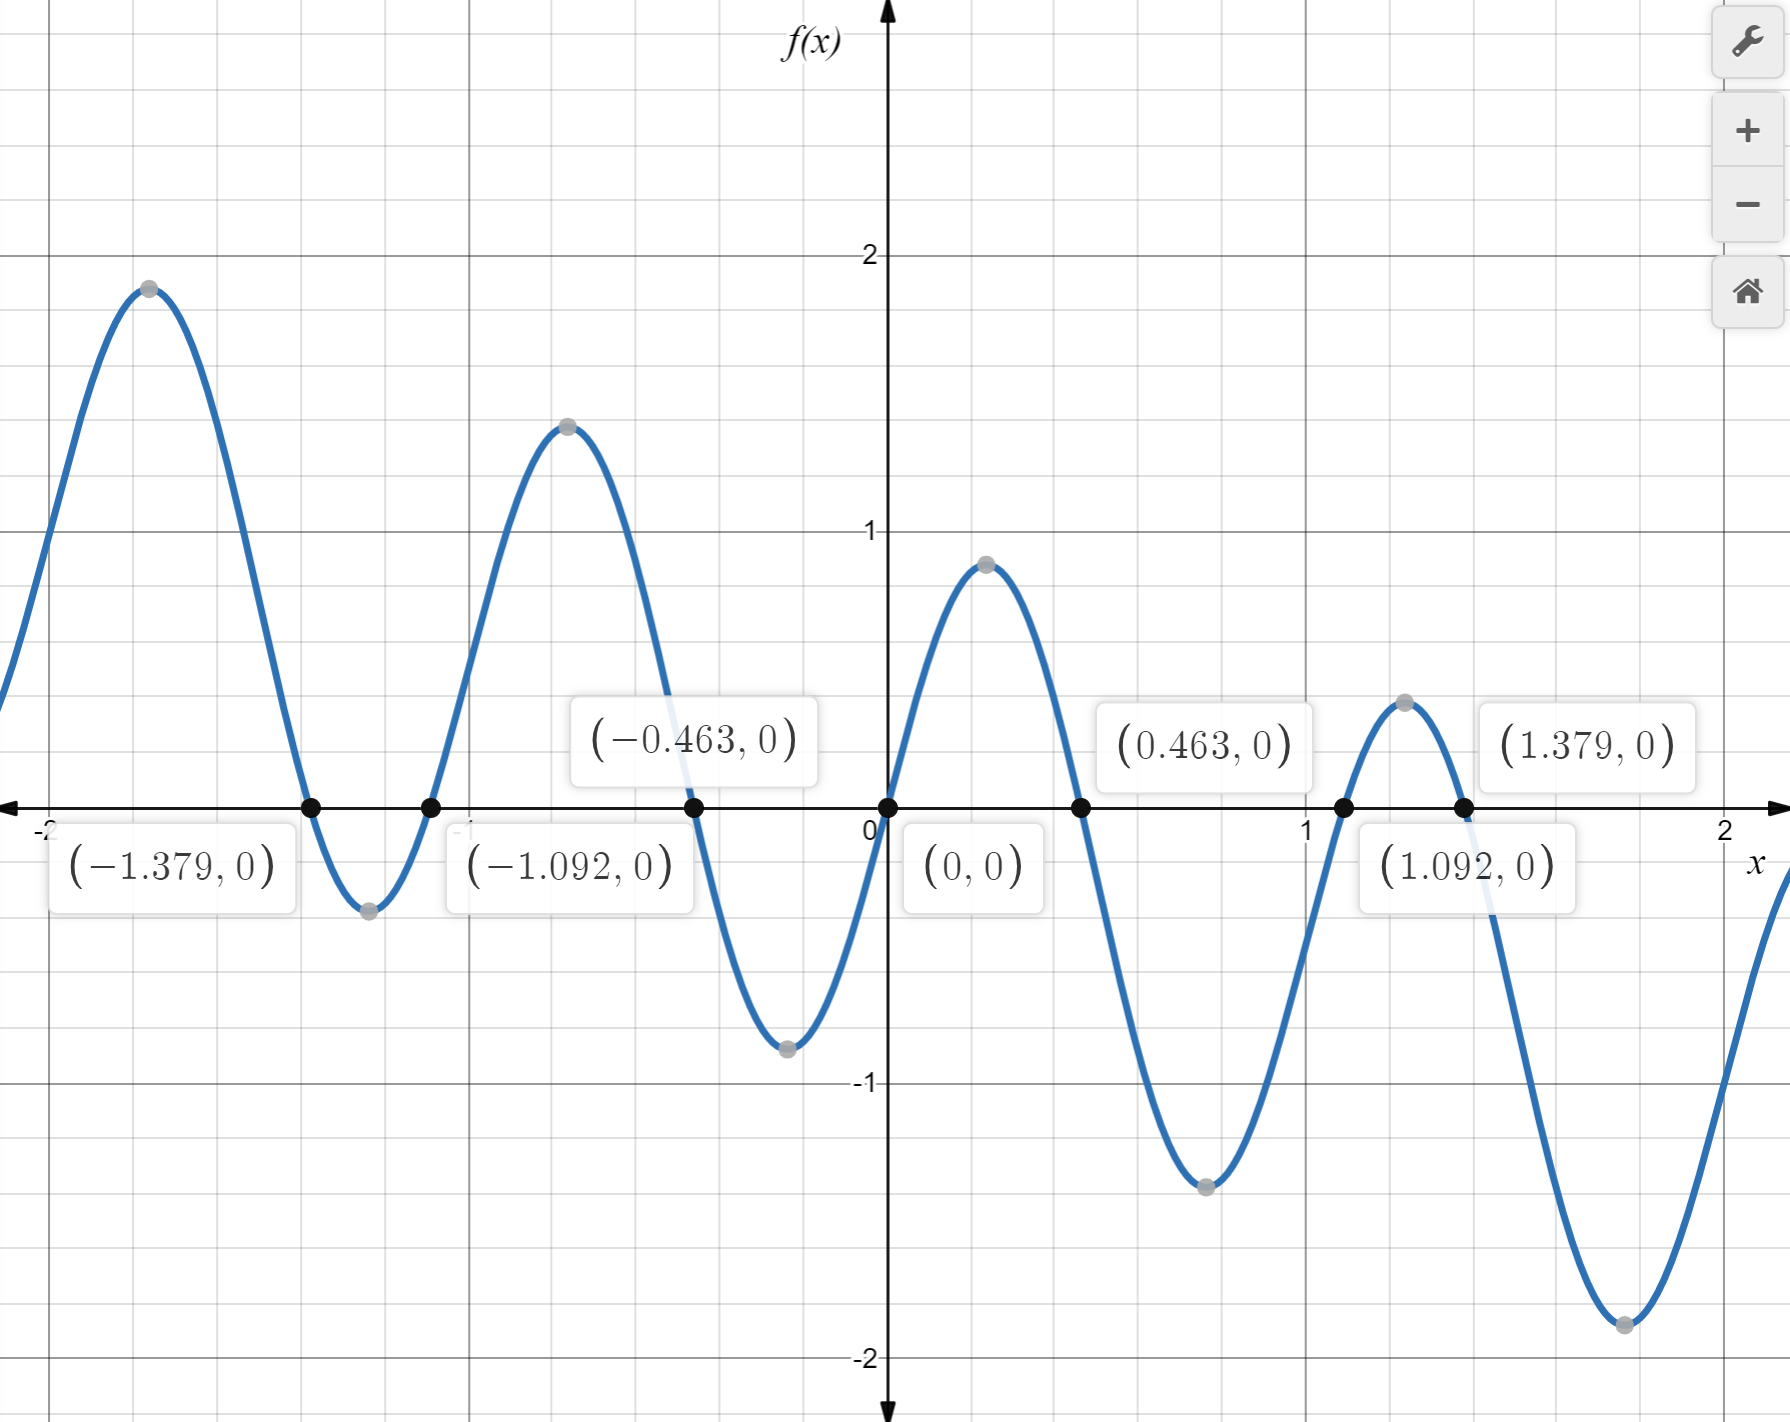
\includegraphics[width=\textwidth]{f3.png}
		\caption{$f(x)=\sin(2\pi x)-0.5x$}
		\label{3e}
	\end{subfigure}
	\caption{Function plots for Problem 3}
	\label{fig:3}
\end{figure}

\subsection*{3(a) Bisection}
In order for Bisection to work, we need to pick two values $x_{low}$ and $x_{high}$ so that $f(x_{low})\cdot f(x_{high})<0$. The range of admissible values for $x$ for the three functions above is summarized in Table \ref{tab:3:1}
	\begin{table}[h]
	\centering
	\begin{tabular}{l c c c }
		\hline
		\hline
		Function & Root &\multicolumn{2}{ c }{Admissible Range} \\
		&&$x_{low}$& $x_{high}$\\
		\hline
		$\sin(2\pi x)-2x=0$	& $x_1=-0.368$&$[-2,-0.368) $&$(-0.368,0)$\\
							& $x_2=0$&$(-0.368,0) $&$(0,0.368)$\\
							& $x_3=0.368$&$(0,0.368) $&$(0.368,2]$\\
		\hline
		$\sin(2\pi x)-x=0$	& $x_1=-0.429$&$[-2,-0.429) $&$(-0.429,0)$\\
							& $x_2=0$&$(-0.429,0) $&$(0,0.429)$\\
							& $x_3=0.429$&$(0,0.429) $&$(0.429,2]$\\
		\hline
		$\sin(2\pi x)-0.5x=0$	& $x_1=-1.379$&$[-2,-1.379) $&$(-1.379,-1.092)$\\
								& $x_2=-1.092$&$(-1.379,-1.092)$&$(-1.092,-0.463)$\\
								& $x_3=-0.463$&$(-1.092,-0.463)$&$(-0.463,0)$\\	
								& $x_4=0$&$(-0.463,0)$&$(0,0.463)$\\	
								& $x_5=0.463$&$(0,0.463) $&$(0.463,1.092)$\\	
								& $x_6=1.092$&$(0.463,1.092) $&$(1.092,1.379)$\\	
								& $x_7=1.379$&$(1.092,1.379)$&$(1.379,2]$\\		
		\hline
		\hline
	\end{tabular} 
	\caption{Polynomial evaluation costs}
	\label{tab:3:1}
\end{table}

\subsection*{3(b) Newton Method}












\section{Question 4}
\begin{enumerate}
\item The linear convergence rate is defined by:
$$\lim_{n \to\infty} \frac{\vert x_{k+1}-x^{*} \vert}{\vert x_{k}-x^{*} \vert} \leq \beta < 1$$\, for some $\beta$.\\
We can rewrite the equation above:

$$
\vert x_{k+1}-x^{*}\vert  \leq \beta \vert x_{k}-x^{*} \vert
$$
Also, We can write the above equation for $x_k$ instead of $x_{k+1}$:
$$\vert x_{k}-x^{*} \vert \leq \beta \vert x_{k-1}-x^{*} \vert
$$
Write recursively:
$$\vert x_{k+1}-x^{*}\vert  \leq \beta \vert x_{k}-x^{*} \vert \cdots \leq \beta^{n+1} \vert x_{0}-x^{*}\vert$$
Hence, the above in equality is the necessary condition for the bisection method to be linearly convergence. In fact, we only can prove the necessary condition but sufficient condition.
\item The bisection method create the nested sequence as follow:
$$[a_n,b_n]\in [a_{n-1},b_{n-1}] \cdots [a_0,b_0]$$
By the construction, we have:
$$a=a_0\leq a_1 \leq a_2 \leq  \cdots \leq a_n \cdots  \leq  b_n \leq \cdots \leq b_2 \leq b_1$$
\item $x_n = \frac{a_n+b_n}{2}$, also $a_n \leq x^* \leq b_n$ for all n.
Implies:
$$\vert x_n -x^* \vert \leq \frac{a_n+b_n}{2} - a_n  = \frac{b_n-a_n}{2}$$
By induction: \\

$$\vert x_n -x^* \vert  \leq \frac{b_n - a_n}{2} =  \frac{b_{n-1} - a_{n-1} }{2^2} =  \frac{b_{n-2} - a_{n-2} }{2^3} =  \frac{b_0 - a_0 }{2^{n+1}}$$
let $\beta = \frac{1}{2}, $$\vert x_0 -x^* \vert  = \frac{b_0-a_0}{2}$, we can prove the necessary condition for the linearly convergence of the bisection method.




\end{enumerate}


\section{Question 5}
The Newton method is given by:
$$x_{k+1} = x_k -\frac{f(x_k)}{f'(x_k)}$$
If $f(x_k) < 0$\\
\begin{enumerate}

\item Case 1: $ x_k < x^* $\\
since $f'(x_k) \neq 0 $
\item Case 1.1: $f'(x_k) > 0 $
Hence, by the newton method recursive equation, we have:
$$x_{k+1} = x_k -\frac{f(x_k)}{f'(x_k)}$$
Since $f(x_k) <0$ and $f'(x_k) > 0 \implies \frac{f(x_k)}{f'(x_k)} < 0 \implies -\frac{f(x_k)}{f'(x_k)}>0$
Let $-\frac{f(x_k)}{f'(x_k)} = \epsilon$\\
The newton equation can be written as:
$x_{k+1} = x_k + \epsilon$ for some $\epsilon >0$, so $x_{k+1}>x_k$ and $f'(x_k) > 0$ the function is strictly increasing, implies $f(x_{k_1}) > f(x_k)$, which is somehow lead us to closer to the root of $f(x)$.

Symestric argument for other cases:

\subsection{Notice}
In the argument above, we rely on the fact that the function f is piecewise monotonic, but in some case, f may behave so that Newton method cannot guide us the the true answer.

ADD PICTURE HERE:




\end{enumerate}




\end{document}

